\documentclass{article}
 
%Russian-specific packages
%--------------------------------------
\usepackage[T2A]{fontenc}
\usepackage[utf8]{inputenc}
\usepackage[russian]{babel}
%--------------------------------------
\usepackage{titlesec}
\usepackage{amsmath}
\usepackage{amssymb}
\usepackage{algpseudocode}
%Hyphenation rules
%--------------------------------------
\usepackage{hyphenat}
\usepackage{graphicx}
\usepackage[left=2cm,right=2cm,
    top=2cm,bottom=2cm,bindingoffset=0cm]{geometry}
\hyphenation{ма-те-ма-ти-ка вос-ста-нав-ли-вать}
%--------------------------------------
\newtheorem{theorem}{Theorem}
 
 
\title{Invertible Residual Networks}
\author{Иван Провилков}
 
\begin{document}
 
\maketitle
%\tableofcontents
 
\section{Введение}
Invertible Residual Network -- архитектура, работающая хорошо одновременно как на дискриминативных, так и на генеративных задачах. Авторы концентрируются на нормализующих потоках и показывают, что заменив нормализацию в ResNet-ах, можно достичь их обратимости.

\section{Нормализующие потоки}

Нормализующий поток это алгоритм, который преобразует плотность начального распределение серией обратимых преобразований в плотность другого распределения. 

Например, если мы генерируем $x$, то можем фактаризовать логарифм правдоподобия:

\begin{equation*}
\begin{aligned}
    \log p_\theta (x) = \log \int p(x|z) p(z) d z = 
    \log \int \frac{q_\phi(z|x)}{q_\phi(z|x)} p(x|z) p(z) d z \geq \mathbb{D}_{KL} [q_\phi (z|x) || p(z) ] + \mathbb{E}_q [\log p_\theta (x|z)] = - \mathbb{F}(x), 
\end{aligned}
\end{equation*}
где $\theta$ - параметры модели, $z$ - скрытые переменные $q_\phi$ - аппроксиматор скрытых переменных. $\mathbb{F}$ (ELBO) -- evidence lower bound, нижняя вариационная оценка. Во время обучения можно оптимизировать ELBO используя различные методы.


\section{Обратимость}

Авторы рассматривают ResNet как Эйлерову дискретизацию обыкновенного дифференциального уравнения:

\begin{equation*}
\begin{aligned}
    x_{t+1} = x_t + g_{\theta_t} (x_t) \\
    x_{t+1} = x_t + h f_{\theta_t} (x_t), 
\end{aligned}
\end{equation*}

где $g$ - residual block, $h$ - step size.

Их интересует обратная динамика: 

\begin{equation*}
\begin{aligned}
    x_{t} = x_{t+1} - g_{\theta_t} (x_t) \\
    x_{t} = x_{t+1} - h f_{\theta_t} (x_t), 
\end{aligned}
\end{equation*}

решение такой динамики позволило бы Residual block-у работать в обратную сторону.

Следующая теорема накладывает достаточные условия для того, чтобы ResNet block был обратимым:

\begin{theorem}
Пусть $F_\theta : \mathbb{R}^d \rightarrow \mathbb{R}^d$ и пусть $F_\theta = (F_\theta^1 \cdot ... \cdot F_\theta^T)$ обозначет ResNet с блоками $F_\theta^t = I + g_{\theta_t}$. Тогда, если $Lip(g_{\theta_t}) < 1, t = 1,...,T$, тогда ResNet обратим. Где Lip(.) - означает константу Липшица.
\end{theorem}

Так как аналитическую форму обратной функции найти сложно, а правая часть уравнения обратной динамики является сжимающей в нашем случае, то авторы используют метод простой итерации для обращения ResNet блока:

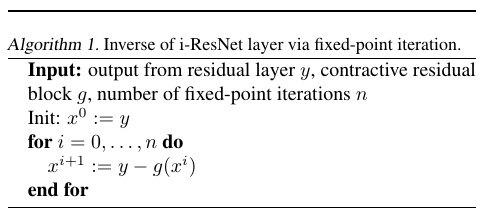
\includegraphics[scale=0.6]{iter_algo.png}.

Согласно теореме Банаха такая итерация имеет экспоненциальную скорость сходимости.

Для того, чтобы ограничение на константу Липшица выполнялось, достаточно сделать спектральную норму весов сверток меньше 1: $g = W_3f(W_2(f(W_1))$, $Lip(g) < 1, $ if $||W_i||_2 < 1$.
Авторы аппроксимируют спектральную норму с помощью метода степенной итерации, а затем нормализуют матрицу используя полученное значение $\sigma_i \leq ||W_i||_2.$

$W_i^{new} = \frac{cW_i}{\sigma_i} I(\frac{c}{\sigma_i}<1) + W_i I(\frac{c}{\sigma_i}\geq1)$, где $c$ -- гиперпараметр. Метод не дает полной гарантии того, что $||W_i||_2 \leq c$, однако авторы делали точный подсчет нормы, и это ограничение на Липшицевость выполнялось в экспериментах. 

\section{Генеративная модель}

Чтобы сгенерировать $x$, вначале генерируется другое распределение $z \sim p_z(z),$ а затем применяется функция $F: x = F(z)$. Для любого $x$ можно рассчитать правдоподобие с помощью формулы замены переменных:

\begin{equation*}
\begin{aligned}
    \ln p_x(x) = \ln p_z(z) + \ln |\det J_{F^{-1}}(X)|,
\end{aligned}
\end{equation*}

где $J_{F^{-1}}$ -- Якобиан обратной функции к $F$.

Так как iResNet обратим, то мы можем использовать его как параметризацию $F^{-1}$. Мы можем сэмплить $z \sim p(z),$ а затем считать $x = F(z).$ 

Главной проблемой в этом процессе является подсчет $\ln |\det J_{F^{-1}}(X)|$, так как явное вычисление этой величины требует $O(d^3)$ времени, где $d$ -- размерность переменной.

С помощью нескольких лемм авторы показывают, что 
$\ln |det J_{F^{-1}}(X)| = tr(\ln J_{F^{-1}})$, в нашем случае $\ln p_x(x) = \ln p_z(z) + tr (\ln (I + J_g(x))). $ 

Нужное нам выражение может быть записано в форме ряда:

\begin{equation*}
\begin{aligned}
    tr (\ln (I + J_g (x))) = \sum_{k=1}^\infty (-1)^{k+1} \frac{tr(J_g^k)}{k},
\end{aligned}
\end{equation*}

который сходится при $||J_g||_2 < 1$. Это условие следует из Липшицевости. 

Аппроксимируя первые члены этого ряда авторы и считают логарифм детерминанта. 

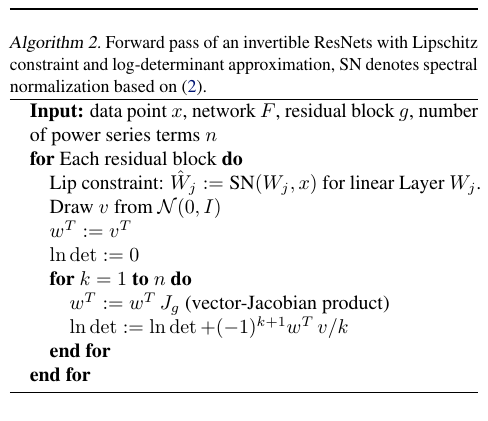
\includegraphics[scale=0.6]{algo_resnet.png}.

\section{Результаты}

Результаты на дискриминативной задаче: 

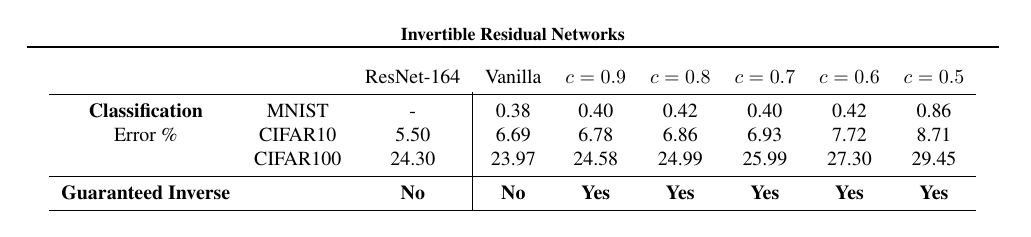
\includegraphics[scale=0.6]{disc_res.png}


Результаты на генеративной задаче:

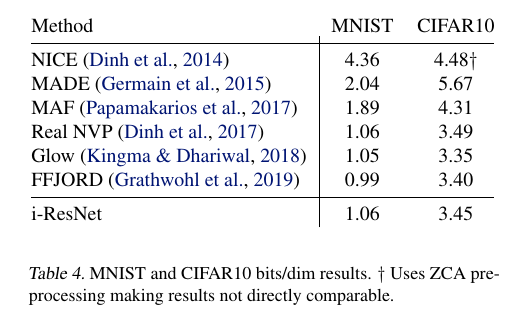
\includegraphics[scale=0.6]{gen_table.png}

Примеры картинок, сгенерированных при обучении на CIFAR10:

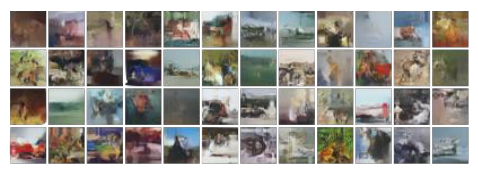
\includegraphics[scale=1.0]{gen_images.png}

\section{Заключение}

В этой статье авторы представили iResNet -- архитектуру, основанную на нормализующем потоке и позволяющую при небольших ограничениях на слои делать интерпретируемую генеративную модель. Эта же модель хорошо показывает себя на дискриминативной задаче, не сильно уступая бейзлайну.



\end{document}
